\subsection{Traffic investigation}
\subsubsection{RF layer}
At the RF layer a few messages can be seen. As shown in the appendix \ref{app:ubertooth} the most packets seen are the NULL and POLL messages. These messages are keep alive messages. During the captures the Ubertooth is only looking at channel 0 on which these packets are sent.
Some other packets are decoded, they are a few of them. These packets contains data and are of type DV/3-DH1, AUX1, AFH, DM1, HV1, DH5/3-DH5. An explanation of these packet types are explained in appendix[?]. The data found have been analysed. The only valuable information that could be output from this data analysis is that the packet are fragmented and seems to be encrypted. Indeed the packets are fragmented as they contain different LLID parameters (which specifies if the payload is the start or the continuation of a L2CAP or LMP message).

\subsubsection{HCI layer}
From the HCI captures, some conclusions can be drawn. Indeed, during the process, some parameters are negotiated regarding the future communication between the two devices. More specifically, what we are looking for are the LMP parameters \ref{fig:lmp}. 

\begin{figure}[!h]
  \begin{center}
	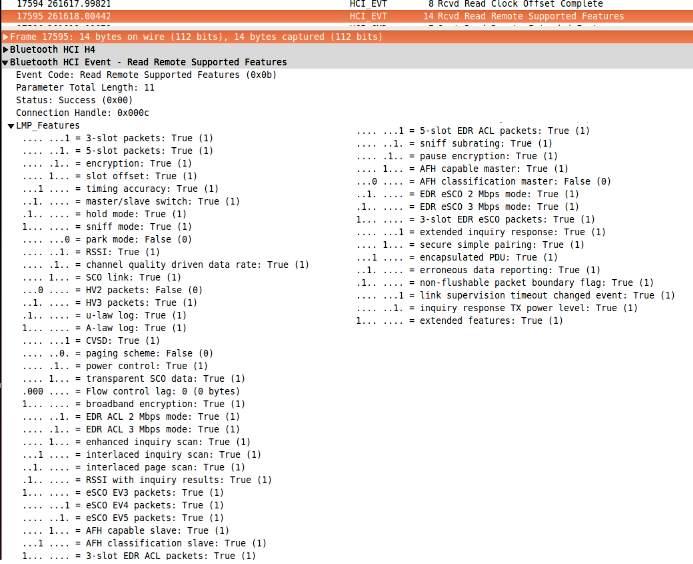
\includegraphics[width=250px]{images/LMP_PARAM.png}
  \end{center}
  \label{fig:lmp}
  \caption{LMP Parameters found during the pairing process at the HCI layer}
\end{figure}

From there, it is true to say that the communication is encrypted, encapsulated and uses SSP. It is even possible to retrieve the link keys used for encryption at this level. The link keys are always updated after a new pairing.

\subsubsection{Correlation of the two layers}

%Why cant we correlate the packet seen on Rf to hci? POLL/NULL-> normal because it is not passing by the hci
%Maybe we should trey to decrypt a packet using the key we found nat the hci. Just to proove that it is possible to decrypt the packets if we would have the key. ANd we would have the key maybe if the ubertooth was doing what we did.

From the pairing process on the HCI, in the connection set up these packet types are disallowed. This is the reason why these packets are not found in the HCI of the master device. As you can see in appendix \ref{app:pairing}. The connection settings are set only to accept these kinds of packets shown. All the packets that are send over this channel which are not poll or null are disallowed types. \pend
The reason why these packets are sent is unknown. 

\subsection{The rogue packets}
As already mentioned, there are some packets we cannot place. These packets can be found by the Ubertooth, but cannot be detected by the HCI. One possibility is that these packets are not meant for the master device. Since the packet types are disallowed by the master it is quite possible, but then the question is why are these sent. Another explanation is that these packets are just the same polling and null packets, but they are just badly decrypted. There is no correlation to be found by comparing the different rogue packets. In fact, there may be some correlation, but it is not clear to guess that by just looking at them as a single set. A possible solution is to have a similar tool as the Ubertooth on the smartwatch to see what is sent at the same time. \\
As seen in appendix \ref{app:roguepackets}, there is an explanation of what information we get about the packet.
Looking at the first packet in appendix \ref{app:roguepackets} there are a few things that can be seen. The data is always doubled and the packet is divided in a few fields. Type, LT\_ADDR, flow, payload length and data where the first line contains some information about the packet. The most important values from this information are:
\begin{itemize} 
\item The \textbf{ch}, this is the channel in which the packet was found.
\item The \textbf{LAP}, which is the sender's lower address part.
\end{itemize}
%Explain the packet. 